\documentclass{article}

\usepackage[utf8]{inputenc}
\usepackage{a4wide}
\usepackage{float}
\usepackage{multirow}
\usepackage{hyperref}
\usepackage{todonotes}

\title{Mapping the Railway formalism onto different domains}
\author{Zhong Xi Lu}
\date{March 2019}

\begin{document}

\maketitle

\section{Introduction}

Modelling is a powerful technique which allows us to work on the right abstraction level and avoid accidental complexity. Nowadays, we have a lot of different formalisms at our disposal, so it's necessary to choose the most appropriate language when building a model. Aside from that, it's also possible to define a mapping from one formalism to another, so that we can expose the functionality of one another.

This paper will revolve around the \textit{Railway} formalism, which is mostly based on \textit{Railway Operation and Control} \cite{railway_book} by \textit{Joern Pachl} and some of the assignments \cite{assignments} given in the \textit{Model Driven Engineering} course in the \textit{University of Antwerp}. This formalism is first modelled in the tool \textit{AToMPM} \cite{atompm} to create a basic visual modelling environment, here we can also simulate a model by defining its operational semantics. To analyze if a model satisfies certain properties, we will map it to petri-nets, where we can do a reachability, coverability, deadlock, ... analysis. Next to that, we can also map it to \textit{Discrete Event System Specifications} (DEVS), which is more appropriate when it comes to queueing, throughput, ... analysis. Finally, to visualize and animate the model, we make use of \textit{Unity} \cite{unity}. \todo{finish introduction}

\todo{add diagram with the different formalisms}

\section{Railway Formalism}

As earlier mentioned, the book \textit{Railway Operation and Control} by \textit{Joern Pachl} \cite{railway_book} was a starting point for this Railway formalism. However, the language used in that book is heavily simplified to make the steps throughout this paper much easier. On top of that, the focus mainly lies on the railway (that consists of different segments) and not much on scheduling, signaling, ... This section will give a brief introduction on this simplified Railway formalism.

At its core, a model consists of multiple segments which can be connected to each other to form a railway. These segments also have a signalling light equipped which will inform an approaching train about its current state: green light means that there's no train represent on the segment and red light means there is. The different types of segments supported by this formalism can be found in table \ref{types_segments}.

\begin{table}[H]
\begin{tabular}{|l|l|l|}
\hline
\textbf{Name:}                 & \textbf{Symbol:} & \textbf{Description:}                                                                                                                                                                      \\ \hline
Straight                       & 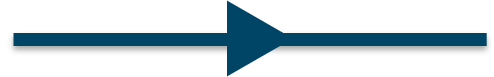
\includegraphics[scale=0.25]{images/straight} & \begin{tabular}[c]{@{}l@{}}a basic segment that connects and is connected\\ by one other segment\end{tabular}                                                                              \\ \hline
Turnout                        & 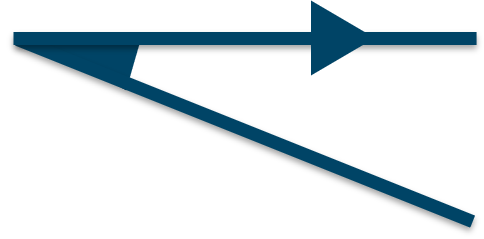
\includegraphics[scale=0.25]{images/turnout1} & \begin{tabular}[c]{@{}l@{}}a segment with internally a switch, which can be\\ used to control its outgoing rail (either going \\ straight or make a turn)\end{tabular}                     \\ \hline
Junction                       & 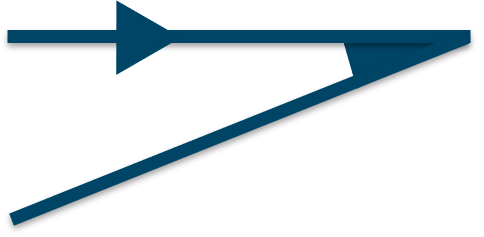
\includegraphics[scale=0.25]{images/junction1} & \begin{tabular}[c]{@{}l@{}}similar to a turnout, but instead of controlling its\\ outgoing rail, it will control the ingoing rail\\ (trains can arrive straight or in a turn)\end{tabular} \\ \hline
Crossing                       & 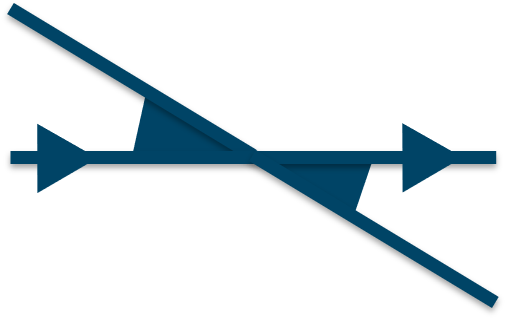
\includegraphics[scale=0.25]{images/crossing21} & \begin{tabular}[c]{@{}l@{}}a combination of a turnout and a junction, has two\\ switches available, allowing to control both the\\ incoming and outgoing rails\end{tabular}                \\ \hline
Station                        & 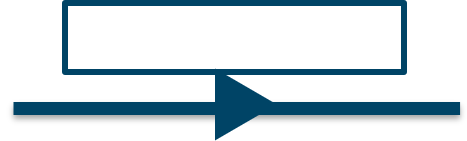
\includegraphics[scale=0.25]{images/station} & a segments with a train station next to it                                                                                                                                                 \\ \hline
\end{tabular}
\caption{All the different types of segments supported by the Railway formalism}
\label{types_segments}
\end{table}

\section{Abstract and Concrete Syntax}

Now that we have defined the initial concepts of our formalism, we can start by building the syntax. This is split in two parts, namely the abstract and concrete syntax. For more information on this topic, I refer to \textit{AToMPM}'s documentation \cite{atompm_docs}.

\subsection{Abstract Syntax}

\begin{figure}[H]
    \begin{center}
        \makebox[\textwidth]{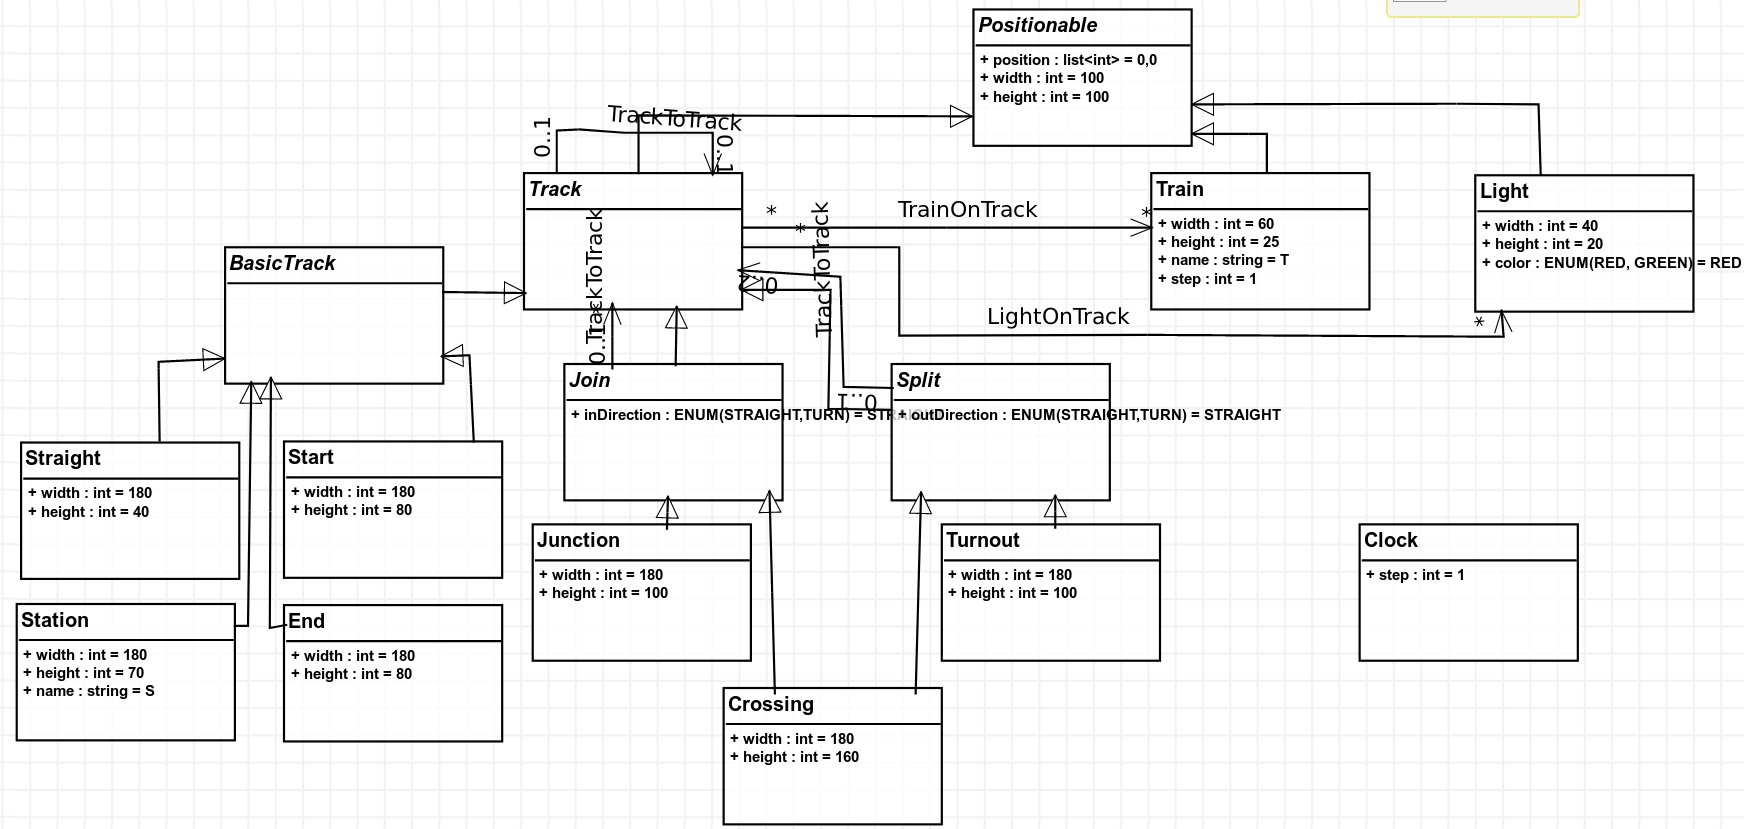
\includegraphics[width=0.9\paperwidth]{images/abstract_syntax}}
    \end{center}
    \caption{Abstract syntax of the Railway formalism}
    \label{abstract_syntax}
\end{figure}

\todo{update figure of abstract syntax}

Since we deal with multiple types of segments, an inheritance tree would be suitable for this problem. At the root, we have an abstract class \texttt{Track}, from here on, we have three (abstract) subclasses:

\begin{itemize}
    \item \texttt{BasicTrack}: All the most basic tracks that have at most one incoming and outgoing track.
    \item \texttt{Join}: A track where two incoming tracks converge, in other words, a junction. It also has an attribute (\texttt{inDirection}) which tells in which the switch is set.
    \item \texttt{Split}: A track that has two outgoing tracks. Similar to \texttt{Join}, this also has an attribute (\texttt{outDirection}) to indicate the current direction of the outgoing track.
\end{itemize}

To actually connect the tracks to one another, the \texttt{TrackToTrack} link is used, by default a \texttt{Track} can only connect and be connected by one other track. However, there are of course segments where this is not the case and where we have to override the existing cardinality constraint constraint; for example, \texttt{Join}s can have two incoming one's and \texttt{Split}s two outgoing one's. This link also has an extra attribute \texttt{direction} to store to which "port" it has been connected in case it's connected to a junction; for example \texttt{STRAIGHT} means that it is connected to the \texttt{STRAIGHT} rail of the junction.

Aside from track, we can also create \texttt{Train}s, which is self-explanatory, and \texttt{Light}s that are used for signalling purposes. These objects can of course be linked and placed on tracks, this is managed by the \texttt{TrainOnTrack} and \texttt{LightOnTrack} links. Finally, a \texttt{Clock} is explicitly modelled here as well, this is to keep track of the simulation steps and make the simulation process easier later on.

Note that there are some "visual" attributes present in the model: \texttt{position}, \texttt{width} and \texttt{height}. These attributes are mainly used to automatically connect segments to each other when they are linked. In true nature, this is not the ideal method to store this in the abstract syntax, but this is just a slight work around to store some visual information. As such, there exists an abstract base class \texttt{Positionable} to deal with this.

\subsection{Concrete Syntax}

\begin{figure}[H]
    \begin{center}
        \makebox[\textwidth]{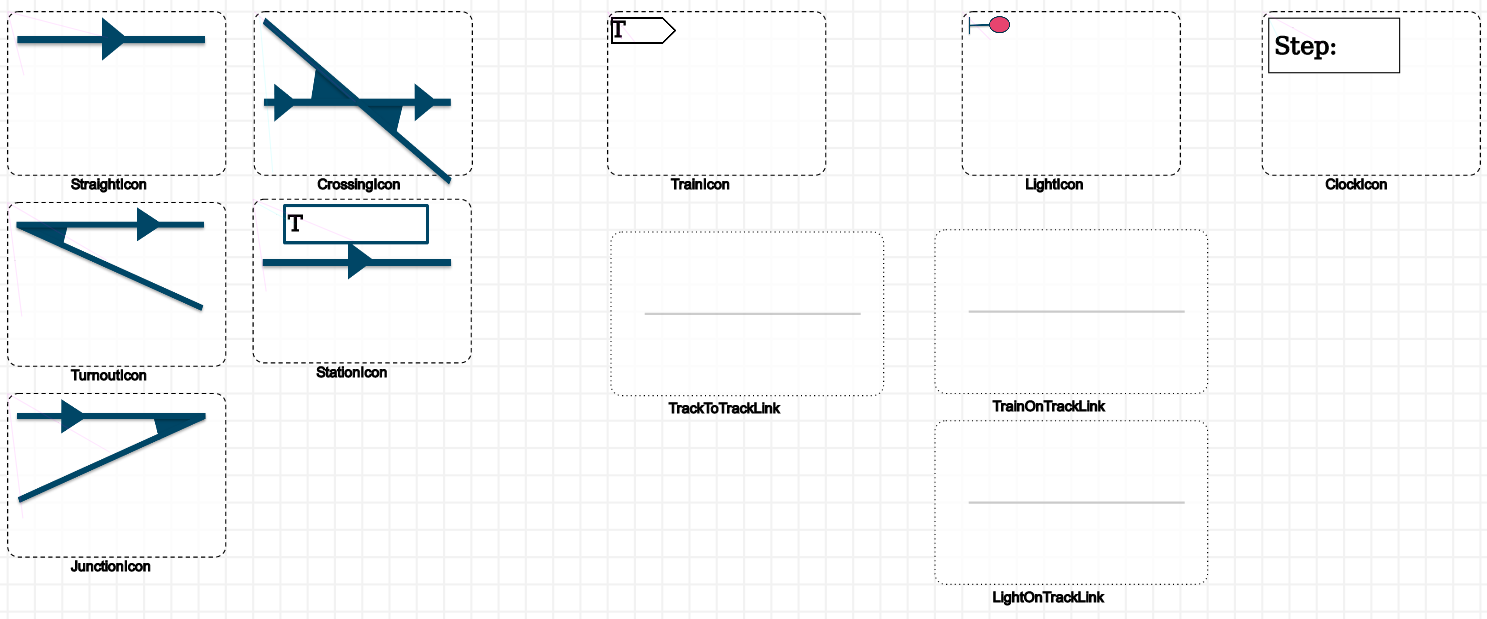
\includegraphics[width=0.8\paperwidth]{images/concrete_syntax.png}}
    \end{center}
    \caption{Concrete syntax of the Railway formalism}
    \label{concrete_syntax}
\end{figure}

Having modelled the abstract syntax, we can now define the icons for our formalism (see figure \ref{concrete_syntax}). Most of these notation are based on the one used in the book \textit{Railway Operation and Control} by \textit{Joern Pachl} \cite{railway_book}. Besides that, these icons also change depending on the state; for example, a junction will show the current direction of the switch (indicated by the arrow). Either way, most these symbols are pretty straightforward.

\section{Operational Semantics}

This section will go over the operation semantics of the Railway formalism, i.e. how the whole system behaves and operates. To model this, we make use of transformation rules, again I refer to \textit{AToMPM}'s documentation \cite{atompm_docs} for more detail.

\subsection{Train Schedule Formalism}

Before we implement the rules, a second domain specific language is modelled to define train schedules (the path it takes from start to end) as was suggested in the \cite{assignments} given in the \textit{Model Driven Engineering} course \cite{assignments}. This way, we can easily operate the switches by looking at the train schedules.

The abstract syntax can be found in figure \ref{abstract_syntax_trainschedule} and the concrete in figure \ref{concrete_syntax_trainschedule}. Basically, a schedule consists of one start station and one ending station. In between are zero or more steps that tell in which direction the train should move when it encounters a waypoint (turnout or crossing). One schedule is associated with  exactly one train and vice versa.

\begin{figure}[H]
    \centering
    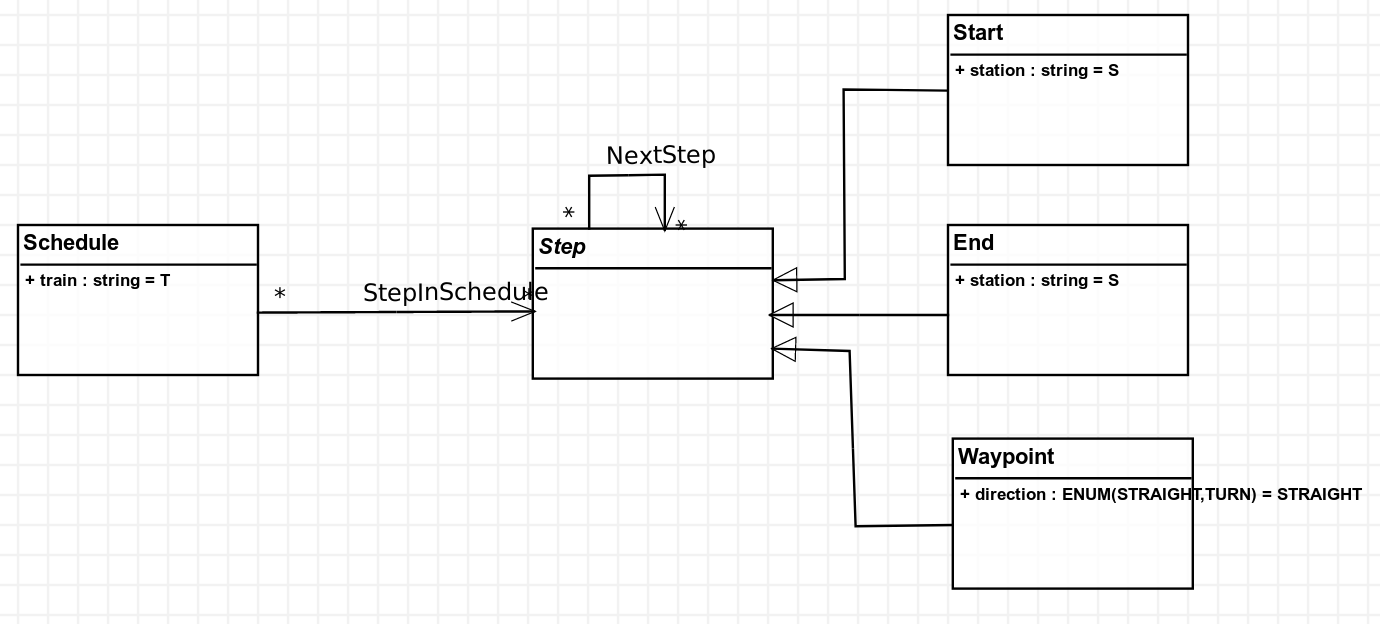
\includegraphics[width=\textwidth]{images/trainschedule_abstract_syntax.png}
    \caption{Abstract syntax of the Train Schedule formalism}
    \label{abstract_syntax_trainschedule}
\end{figure}

\begin{figure}[H]
    \centering
    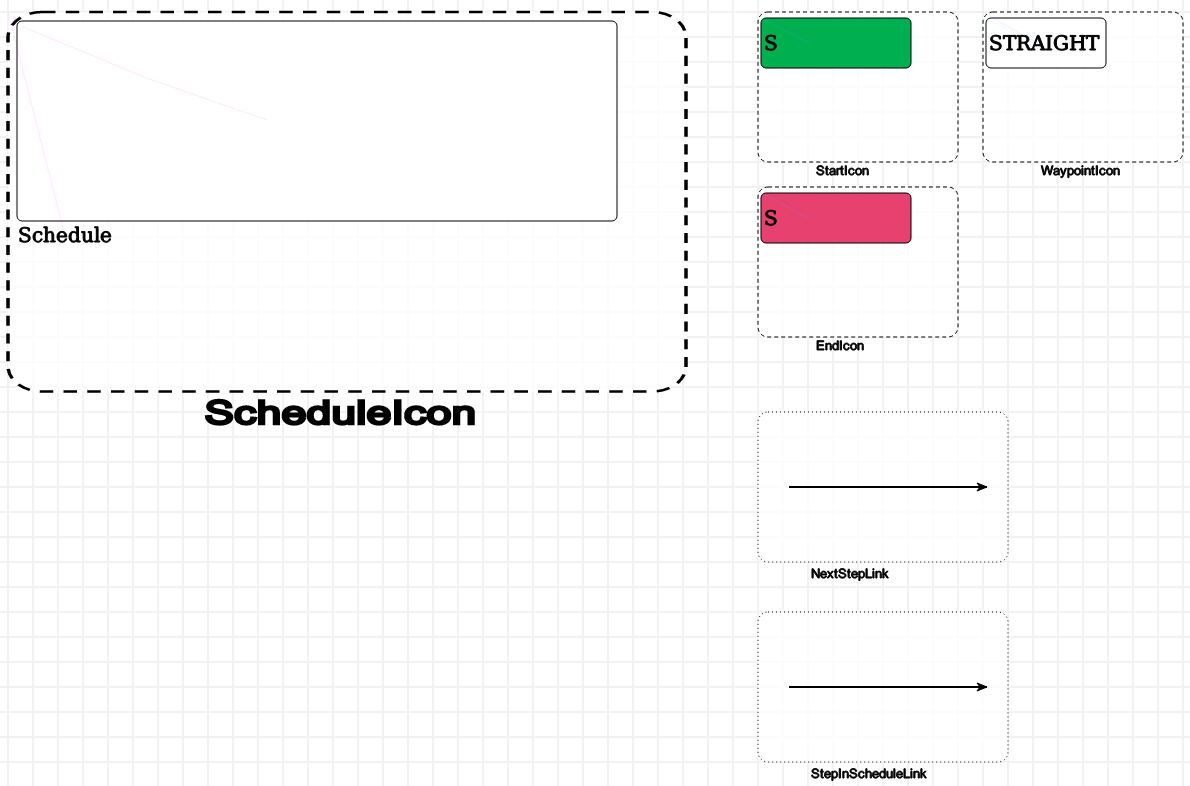
\includegraphics[width=\textwidth]{images/trainschedule_concrete_syntax.png}
    \caption{Concrete syntax of the Train Schedule formalism}
    \label{concrete_syntax_trainschedule}
\end{figure}

\subsection{Operational Semantics}

\begin{figure}[H]
    \centering
    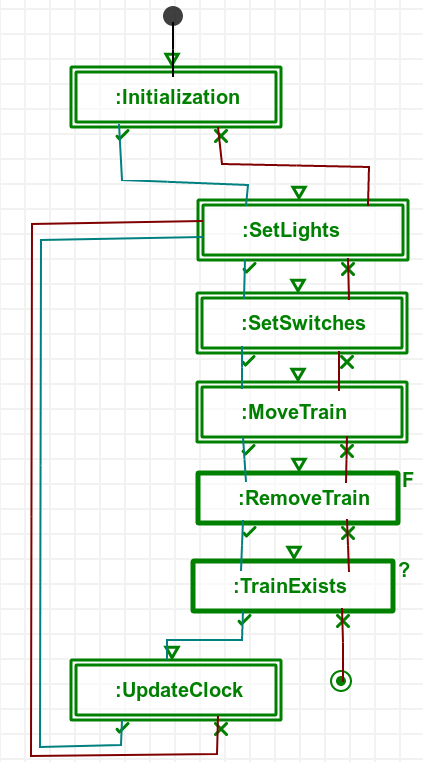
\includegraphics[width=0.4\textwidth]{images/schedule_opsem.png}
    \caption{Schedule for the operational semantics}
    \label{schedule_opsem}
\end{figure}

To explain the semantics, I will go over the MoTif schedule (figure \ref{schedule_opsem}):

\begin{enumerate}
    \item Initialization: Adds signalling lights to all tracks if that wasn't the case already and it will place all the trains on their starting station according to their unique train schedule.
    \item Set Lights: Set the lights correctly depending on their state; set the light green if there's no train present and red otherwise.
    \item Set switches: Set the switches on splits and joins:
        \begin{itemize}
            \item Joins: if a train wants to enter a junction, the control system will set the direction of the incoming track correctly so that the train can enter. If two trains want to enter, it will "randomly" choose one.
            \item Split: to set the switch for splits, we look at the train schedule of the train that is currently on this split. This schedule will tell us in which direction we should move. We then remove that step, indicating it was taken. (see figure \ref{set_split_switch})
            \begin{figure}[H]
                \centering
                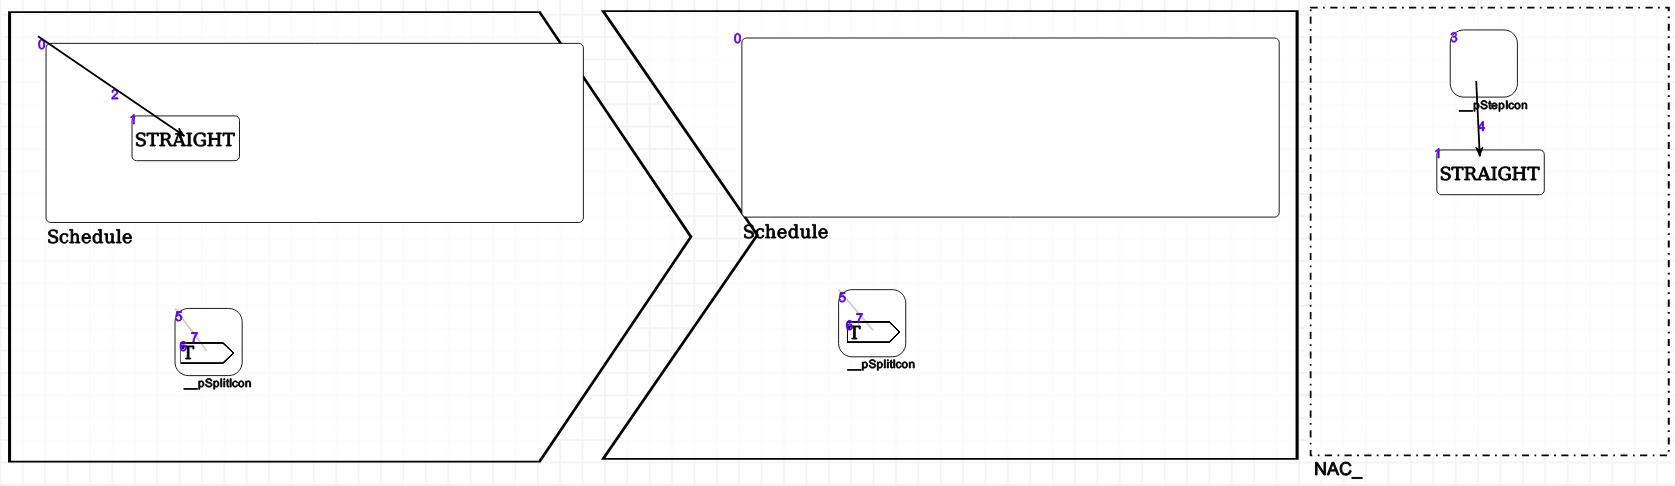
\includegraphics[width=\textwidth]{images/SetSplitSwitch.png}
                \caption{Transformation rule for setting switch on splits}
                \label{set_split_switch}
            \end{figure}
        \end{itemize}
    \item Move Train: This step will try to move a train to the next segment. There are however several cases that we have to keep in mind; for example, we can only move if the light on the next section is green. Most of these cases verify if the in/out-direction is set correctly.
    \item Remove Train: Whenever a train reaches its end (station), we will remove it from the model, so that potential future train can enter this station as well.
    \item Train Exists: A simple query rule to check if there are still trains left on any track. This is the end condition and the transformation will halt if there cannot be a train found.
    \item Update Clock: Finally, if the \texttt{TrainExists} was successful, we can move to the next simulation cycle: this step will update the clock as well as the step internally of all the trains so that they are synchronized with the clock.
\end{enumerate}

\section{Safety Analysis}

Given a model written in our railway formalism, one would also want to do some analysis regarding its safety, for example if there is a reachable deadlock state. To do all this, we can define a mapping (using transformation rules) to petri-nets. These nets are highly suitable to these kinds of analyses. In this case specifically, the tool \textit{LoLA} (\textit{a Low Level Petri net Analyzer}) \cite{lola} will be used to analyze a given petri-net by building the reachability graph etc.

\begin{figure}[H]
    \centering
    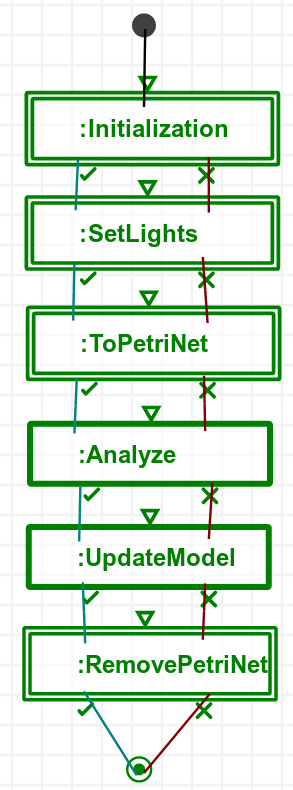
\includegraphics[width=0.25\textwidth]{images/analyze.png}
    \caption{Schedule for the safety analysis}
    \label{schedule_safety}
\end{figure}

The full MoTif schedule for the safety analysis can be found in figure \ref{safety_analysis}. First, we initialize the model so the trains are on the right tracks and the lights are all correctly set. Then we actually do the petri-net mapping and finally we can analyze the intermediate petri-net with a few LoLA calls and update the railway model if that's necessary.

This section is divided in three parts; section \ref{petri-net_mapping} will define the mapping itself, section \ref{safety_analysis} will discuss some "safety" properties and how we can define those in \textit{LoLA} and finally, in section \ref{safety_updating} will go over how we can use the results generated by \textit{LoLA} to update our initial model to show it to the user.

\subsection{Mapping}
\label{petri-net_mapping}

The complete mapping is fairly trivial and can be split in several steps/rules:

\begin{itemize}
    \item Tracks become places. If one contains a train, the place has a marking value of $1$.
    \item Links between tracks (\texttt{TrackToTrack}) become transitions. Note that when a train goes from one track to another, it will also look at the places that correspond to the lights (see next point).
    \item Lights can be split up in two places: one for the green color and one for the red color. This will mean that at all time the sum of these places will always be equal to $1$.
    \item To make sure the petri-net can go on forever, we add one additional place for each end station in a train schedule and one transition that will take all the tokens in those places and put them back. This means that if all the trains have reach their end station, this transition can fire an infinite amount of times.
\end{itemize}

Combining all these rules, we now have an analyzable petri-net that represents the Railway formalism.

\subsection{Analysis}
\label{safety_analysis}

On this petri-net, we can run several analyzes using \textit{LoLa} to verify if the model satisfies a particular property.

\subsubsection{Deadlock}

A simple property is deadlock; we want to be able to verify if there is a reachable deadlock state from the start state. If there is any, the user may want to change the initial model to prevent this from happening. In this context, a deadlock means that it is possible for a train to get stuck somewhere in the railway network and never get moving again, which is of course not what we want. This property will also implicitly tell us whether the trains can all reach their end station.

\subsubsection{Reachability}

Petri-nets are highly suitable for reachability analysis, more specifically, with this we can verify if a specific place is reachable from the the initials state. In other words, tracks that cannot be reached by a train (in the initial setup). For this, we make $n$ LoLA calls ($n$ = number of tracks) where we check each time individually if that track can be reached.

\subsubsection{Safeness}

Since we're dealing with trains on rails, it's of course desirable to have that trains cannot crash into each other, i.e. two trains on one single track. To verify this, we can check if our whole petri-net is 1-bounded or safe, meaning in every place there cannot be more than one token or on every track there can be at most one train present.

\subsubsection{Lights Invariant}

In our petri-net mapping, we introduced two places for each signalling light. Implicitly, this means that only one token can be in those two places combined or else the lights are both green and red (or neither of them are on). This property will then check if at all time the sum of two places (of a light) is equal to $1$ (invariant).

\subsection{Updating model}
\label{safety_updating}

When analyzing and finally generating the results, we want to be able to show them to the user somehow. The way we do this is also through a small model transformation that reads those results in and updates the railway model accordingly. For example, highlight (and add a few comments about) the path that led to a deadlock state.

One important thing to note is when mapping the results (of the analysis) back to our original model, we need some form of traceability. We can create traces by making use of unique identifiers for the objects in the railway model and then use the same ones in the petri-net model. This way, we can correspond a petri-net element to its original element.

\todo{add reference to appendix?}

\section{Queueing Analysis}

Another analysis we can perform is queueing analysis, for example, how long it averagely takes for a train to reach its end station or how long a train has to wait to enter its next segment. To do this, we create another mapping, this time we map the Railway formalism to DEVS. Here we can simulate a given DEVS model and retrieve the necessary information from it. The DEVS library used for this is \textit{PythonPDEVS} \cite{pythonpdevs}.

\begin{figure}[H]
    \centering
    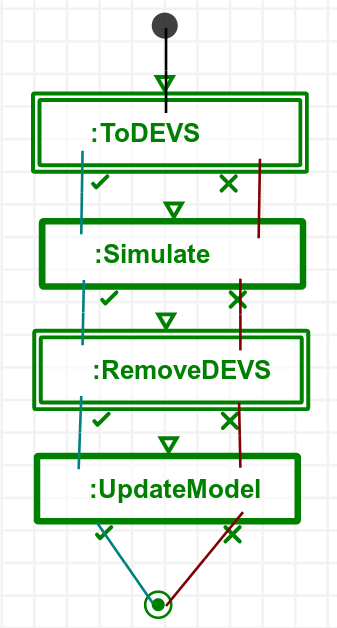
\includegraphics[width=0.25\textwidth]{images/queueing_analysis_schedule.png}
    \caption{Schedule for the queueing analysis}
    \label{schedule_queueing}
\end{figure}

\subsection{Mapping}

When mapping the Railway elements to DEVS elements, one must specify the DEVS model as well. For instance, we need a DEVS model for a track that describes its behaviour. One such model has different components, such an internal transition function, states, output function, etc. However, I did not choose to take this path, instead I already had these models implemented with the \textit{PythonPDEVS} library, so I saved myself some time, but ideally one should also model this (in \textit{AToMPM}). I will not go in further details on the semantics of the DEVS models, but more on how I implemented these can be found in the DEVS assignment, part of the \textit{Modelling of Software-Intensive Systems} course \cite{devs_assignment}.

Either way, we still need to create instances of these DEVS models and encapsulate them in a coupled DEVS and of course, we use transformation rules yet again to transform our railway model. Similarly to the petri-net mapping, we can define some basic rules that will take care of this mapping:

\begin{itemize}
    \item Tracks become DEVS instances. There are four main DEVS models, namely \texttt{RailwaySegment}, \texttt{Join}, \texttt{Split} and \texttt{Crossing}. Most of these instances also link to in- and out-ports. The in-ports are \texttt{train\_in}, \texttt{Q\_recv} and \texttt{Q\_rack} and the out-ports \texttt{train\_out}, \texttt{Q\_send} and \texttt{Q\_rack}. What these ports specifically mean, I refer to the DEVS assignemnt \cite{devs_assignment}. Note that some of these models can have more ports, depending on their type; for example, a split will have a \texttt{train\_out} and \texttt{train\_out2} port.
    \item Links between tracks (\texttt{TrackToTrack}) become so-called channels which connect to in- and out-ports.
    \item Since we are performing a queueing analysis, we most likely want more than a few trains in our network. Hence, there is also a \texttt{Generator} DEVS model; this will generate trains following an inter arrival time distribution. This way, a more in depth analysis can be performed and trains actually get queued. The railway element that gets mapped to this generator is the \texttt{Station} that is also the start (station) of a train schedule.
    \item On the other hand, a \texttt{Collector} is also represent. This will simply remove a train object and store some statistics. Here, the \texttt{Station} that corresponds to an end station of a schedule will get translated to this collector element.
\end{itemize}

\subsection{Analysis}

Simulating a complete coupled DEVS model with \textit{PythonPDEVS} will create a detailed trace that specifically tells us at each point in time what has happened, but to retrieve more information, we need to add more logic to the models, but this is quite easily done. On top of that, there some extra attributes in the abstract model (e.g. segment length, train acceleration, ...), so that the user can manually (or by script) tweak the settings and try to optimize a given railway model. In the following small subsections, the few statistics integrated are discussed.

\subsubsection{Average Transit Time of a Schedule}

In the railway formalism we allowed to the user to define the schedule for a particular train, but it might also be interesting to see if the schedule is actually effective, i.e. getting fast from the start station to the end station and having to wait minimally. Maybe some schedules are interfering with each other, i.e. a train has always to wait for another train (some sort of priority), so knowing the actual transit time can be quite useful. To retrieve this information, we add an extra attribute to a train, namely the train's departure time and when a train arrives at its end station (i.e. a collector), we can subtract the current time with that departure time. At the end of the simulation, we can take the average of all the transit times to get the final result.

Next to this, we can also show the number of trains that have been generated (at their start station) and that have arrived to their destination, this can then also tell us whether all the trains seemingly can drive to their end location.

\subsubsection{Throughput and Average Transit Time of a Railway Segment}

It might also be interesting to look at an individual segment instead of the complete schedule. In such manner, we can isolate single tracks and look at their own performance. First, we can record the time that a train needs to pass through this segment. This implicitly also says whether a train has to wait a lot while being on this segment. Knowing this, we can try to avoid this by changing the initial schedule and for instance, take another route.

Secondly, we can also store a track's throughput, i.e. the percentage that a train is present on the track. Generally, having a higher throughput is better, but together with the average time to pass this segment, one might expose some conjunction points in the railway network. For example, a certain junction has a high throughput which might mean that trains get clustered before that junction. Additionally, the mount of trains that passed this section is also kept, so we can easily track the trains.

\subsection{Updating Model}

Like with safety analysis, we update our initial railway model with the gathered results from the DEVS simulation. Again, we make use of id's to have backward traceability, so we can precisely relate the results to a track.

\section{Conclusion}

\bibliographystyle{ieeetr}
\nocite{*}
\bibliography{references}

\newpage
\section*{Appendix: Examples}
\label{appendix}

\subsection*{Operational Semantics}

\begin{figure}[H]
    \centering
    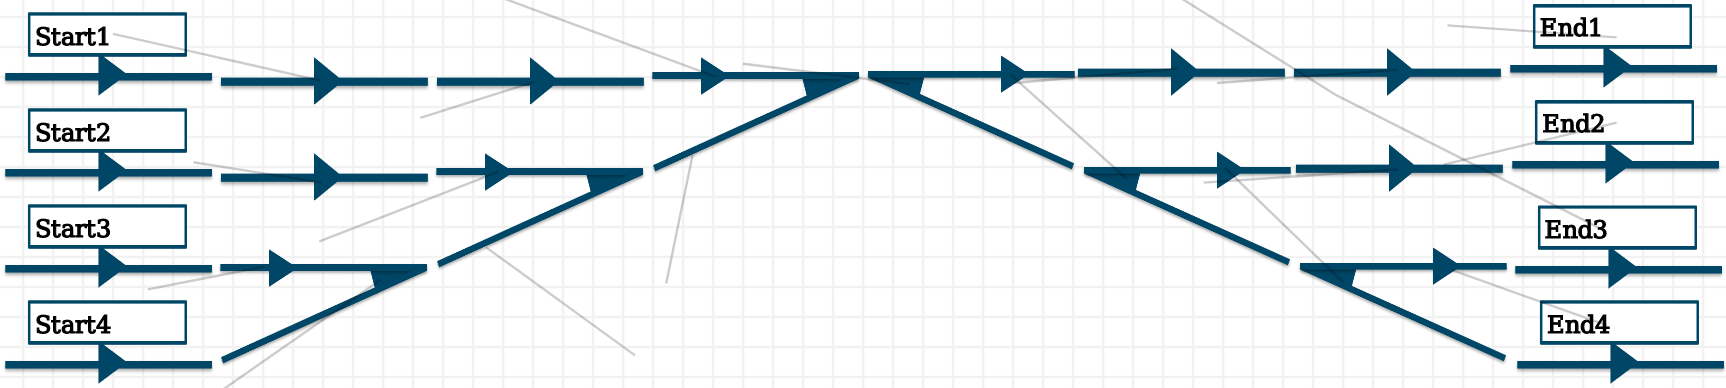
\includegraphics[width=\textwidth]{images/example_devs_railway.png}
    \caption{Railway model for the operational semantics}
    \label{example_devs_railway}
\end{figure}

\begin{figure}[H]
    \centering
    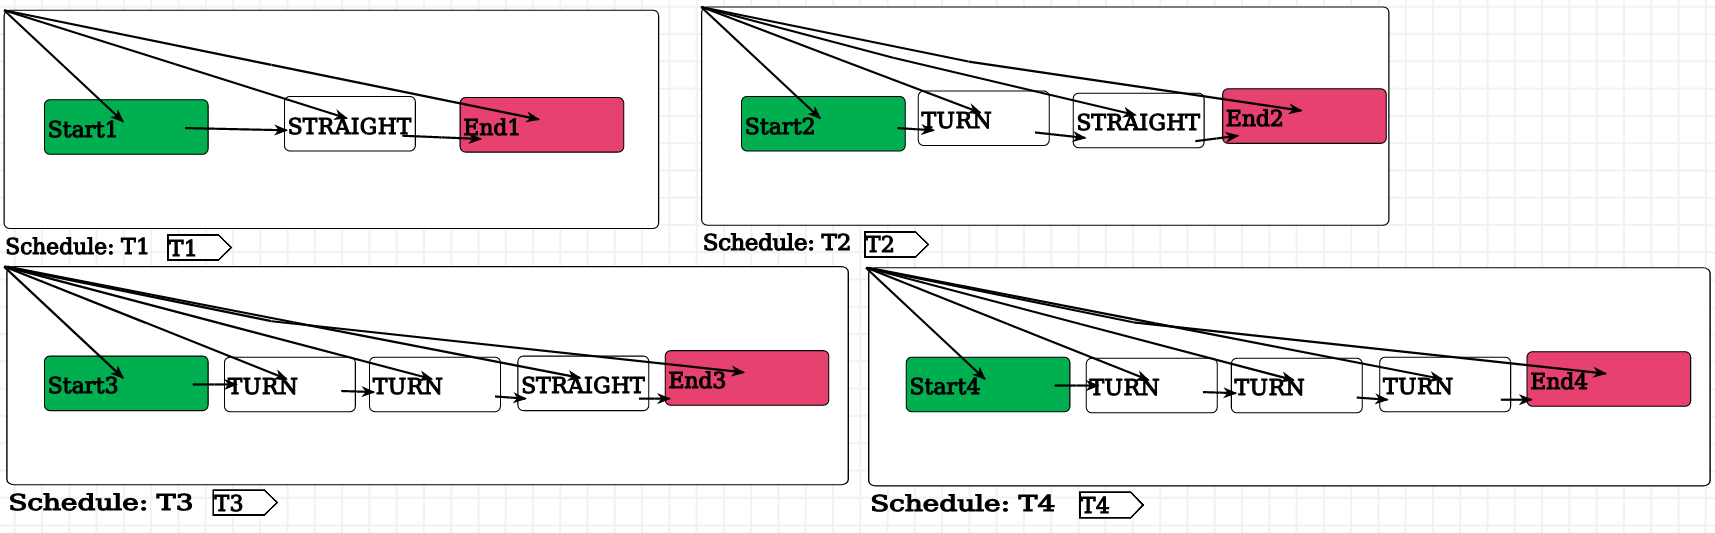
\includegraphics[width=\textwidth]{images/example_devs_schedule.png}
    \caption{Train schedule models for the railway model in figure \ref{example_devs_railway}}
    \label{example_devs_schedule}
\end{figure}

The example model we will be working on for the operational semantics is shown in figure \ref{example_devs_railway}. The small network consists of four start and end stations that are connected to some sort of ladder. For each start station we also associate exact one train schedule, which can be found in figure \ref{example_devs_schedule}. For example, train \texttt{T1} has to continuously go straight, while \texttt{T4} always has to take a turn on a turnout.

\begin{figure}[H]
    \centering
    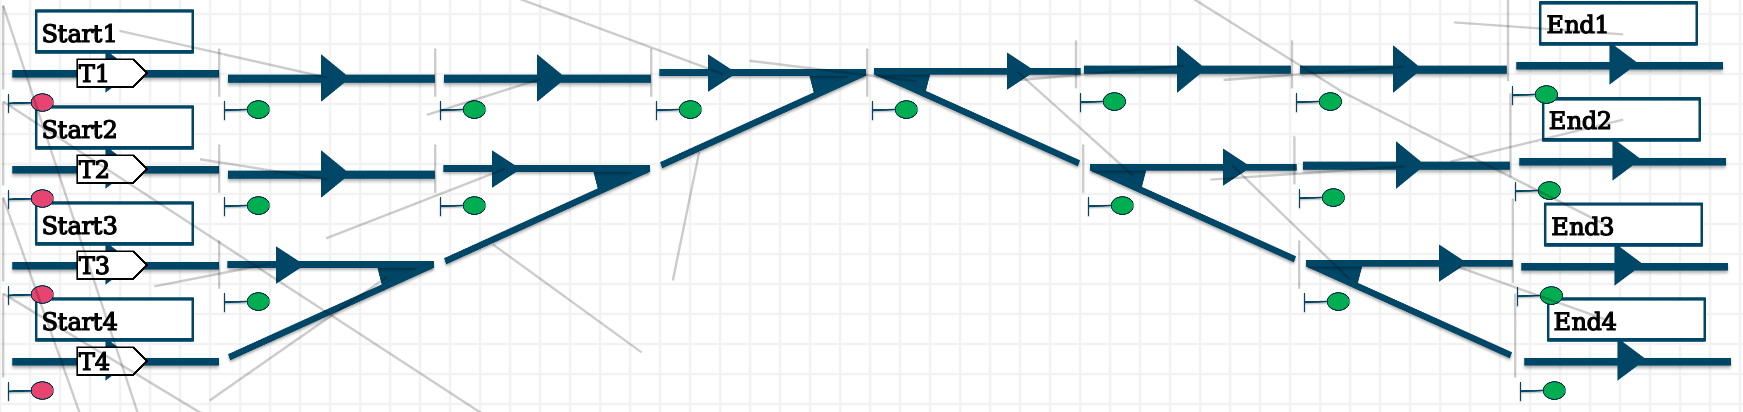
\includegraphics[width=\textwidth]{images/example_devs_after_init.png}
    \caption{Model after initialization}
    \label{example_devs_after_init}
\end{figure}

After the initialization (figure \ref{example_devs_after_init}), all the trains are placed on their start station and all the signalling lights are added and set correctly.


\begin{figure}[H]
    \centering
    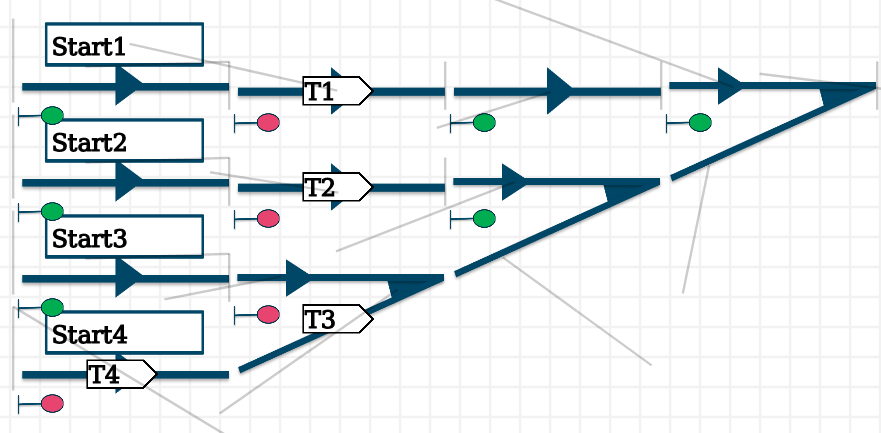
\includegraphics[width=0.6\textwidth]{images/example_devs_after_first_iter.png}
    \caption{Model after first iteration}
    \label{example_devs_after_first_iter}
\end{figure}

After the initialization, the real simulation loop can start. The first iteration (figure \ref{example_devs_after_first_iter}) starts by setting the switches, in this case, only one switch (most bottom junction) will be set. There are however two trains (\texttt{T3} and \texttt{T4}) who want to enter this junction, so it will randomly select one (\texttt{T3} here). After this step, the trains can try to move to the next segment, all the trains can move, except \texttt{T4} since the switch of the junction is not set correctly.

\begin{figure}[H]
    \centering
    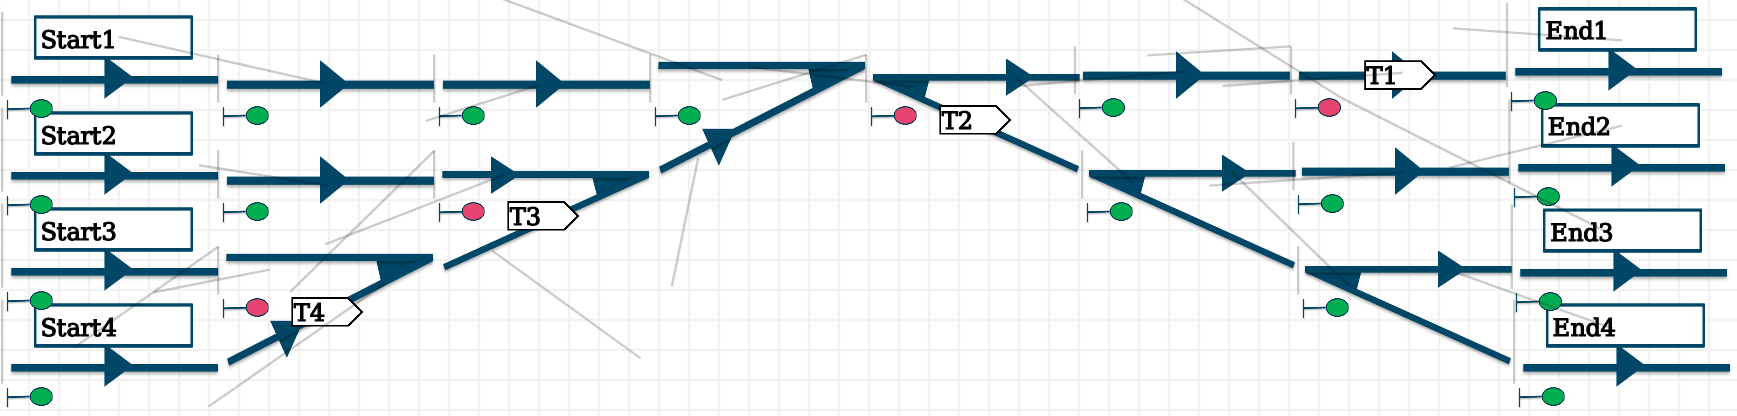
\includegraphics[width=\textwidth]{images/example_devs_after_few_iters.png}
    \caption{Model after several iterations}
    \label{example_devs_after_few_iters}
\end{figure}

If we let the simulation run several iterations, we come to the following model in figure \ref{example_devs_after_few_iters}. Interestingly enough, \texttt{T1} is almost already at its destination, while \texttt{T4} just left its start station. This is due to the fact that \texttt{T1} only has to enter one junction (more on this in the \nameref{queueing_analysis_section} section). Finally, if we let the simulation run until the end, \texttt{T1}, \texttt{T2}, \texttt{T3} and \texttt{T4} will eventually reach their end location in this order.

\subsection*{Safety Analysis}

\begin{figure}[H]
    \centering
    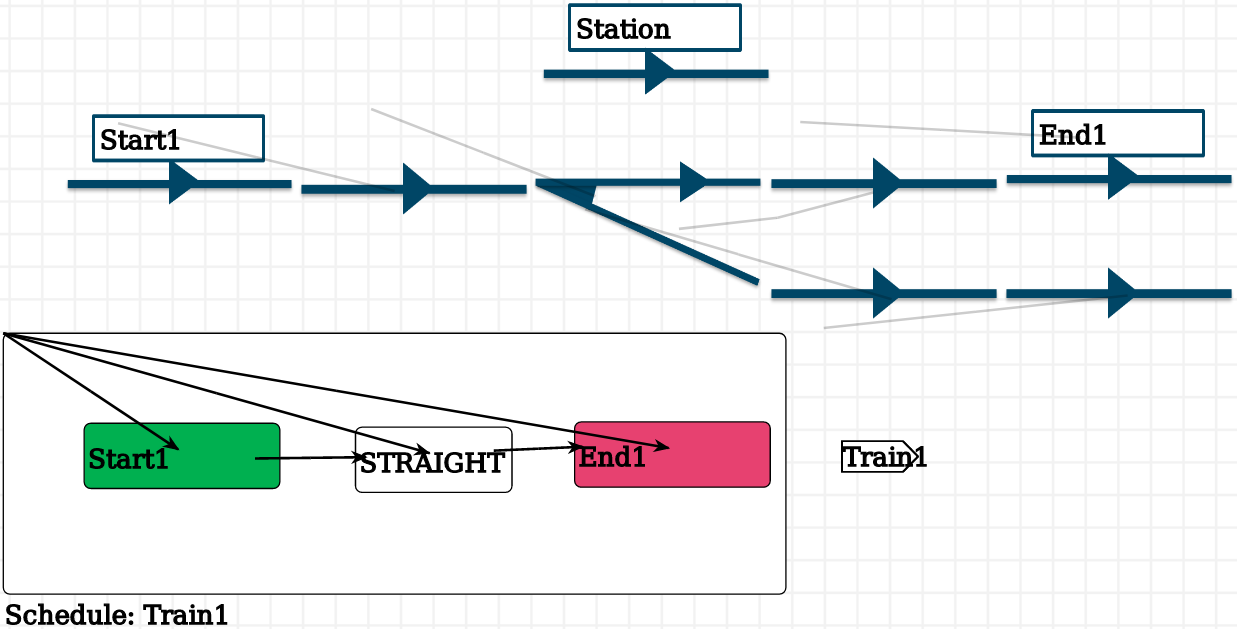
\includegraphics[width=\textwidth]{images/example_pn.png}
    \caption{Railway and Train Schedule Model for the safety analysis}
    \label{example_pn}
\end{figure}

The model that we will be analyzing is pictured in figure \ref{example_pn}. It contains only one train of which its schedule is simply going straight until it reaches its end station.

\begin{figure}[H]
    \centering
    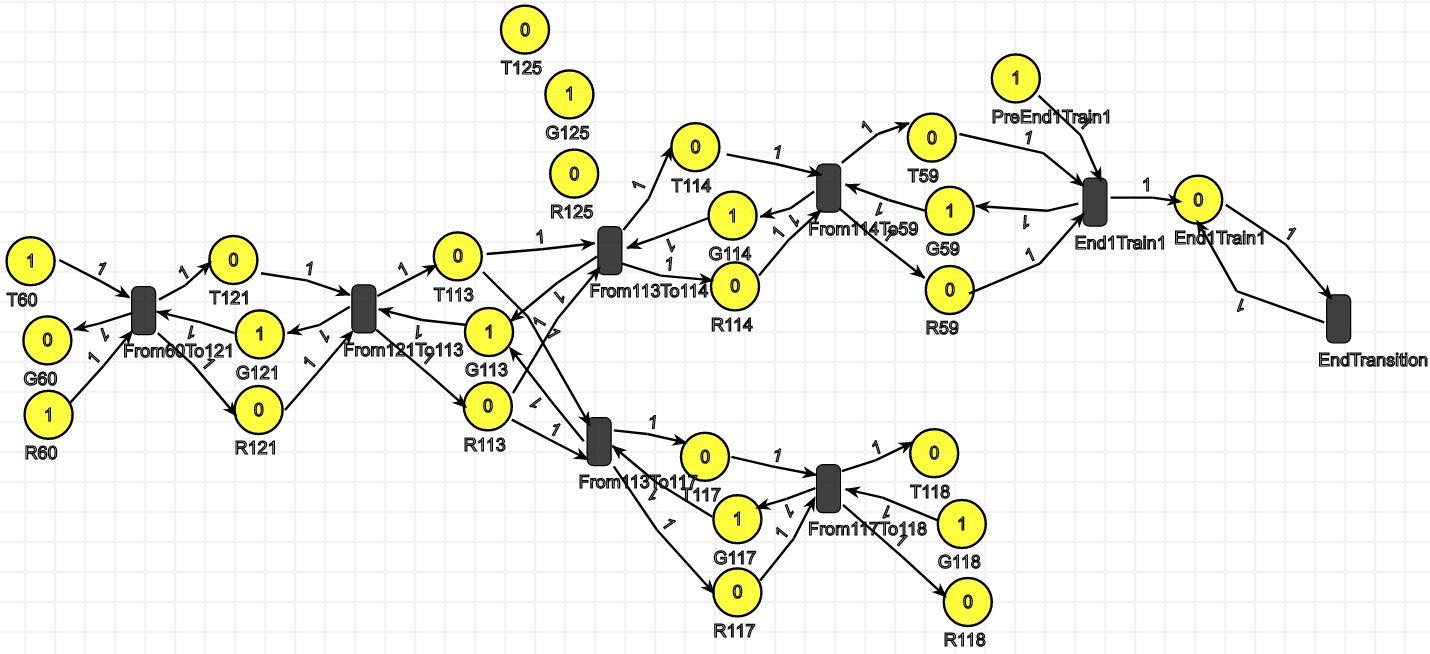
\includegraphics[width=\textwidth]{images/example_pn_pn.png}
    \caption{Intermediate petri-net model}
    \label{example_pn_pn}
\end{figure}

When running the model transformations, an intermediate petri-net model is created, this can be viewed in figure \ref{example_pn_pn}. All of the tracks have three places, one for the actual track and two for the light. For each end station (of a schedule) we also associate one place (here it is \texttt{End1Train1}) where the train resides after it has reached its end station. Note that the \texttt{PreEnd1Train1} place holds one token, so that only one train finish in this station. Finally, if the end condition is met (all trains are in their end station), the \texttt{EndTransition} will then infinitely be enabled and fired.

\begin{figure}[H]
    \centering
    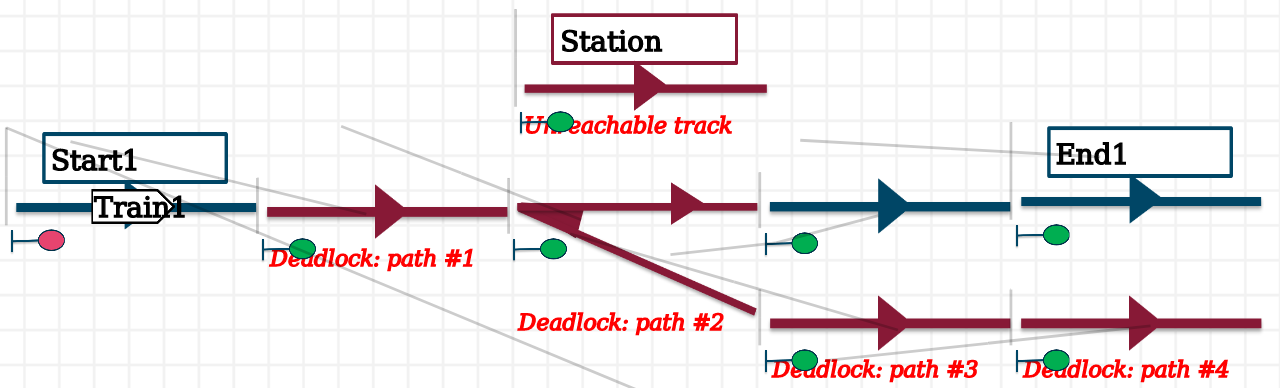
\includegraphics[width=\textwidth]{images/example_pn_results.png}
    \caption{Safety analysis results}
    \label{example_pn_results}
\end{figure}

From this intermediate petri-net, we can run our analysis and import the results back onto our railway model. The effect of this can be seen in figure \ref{example_pn_results}. First, there is an unreachable station \texttt{Station} and secondly, it might be possible to end up in a deadlock situation if we follow the indicated path on the model, i.e. instead of going straight on the turnout, the train takes a turn and goes into a dead path. Note that in practise this should not be possible if the control system is functioning correctly, i.e. setting the switch on the turnout according to a train's schedule.

\subsection*{Queuing Analysis}
\label{queueing_analysis_section}

For the queueing analysis, we start off with the same model we used for the operational semantics (figure \ref{example_devs_railway} and \ref{example_devs_schedule}). Note that the railway segments are all five kilometers long, the inter arrival time (IAT) for all the generators are $[5,10]$ seconds, the train's acceleration is $[0.2,0.7] m/s^2$ and the simulation runtime is 100.000 seconds (or roughly 28 hours). We make the inter IAT short enough so that trains can get queued, so we can see how the train system will function under heavy load. As earlier mentioned, we could already tell that \texttt{T1} reached its end station way before the others, but to go deeper on this, we can make use of the queueing analysis.

\begin{figure}[H]
    \begin{center}
        \makebox[\textwidth]{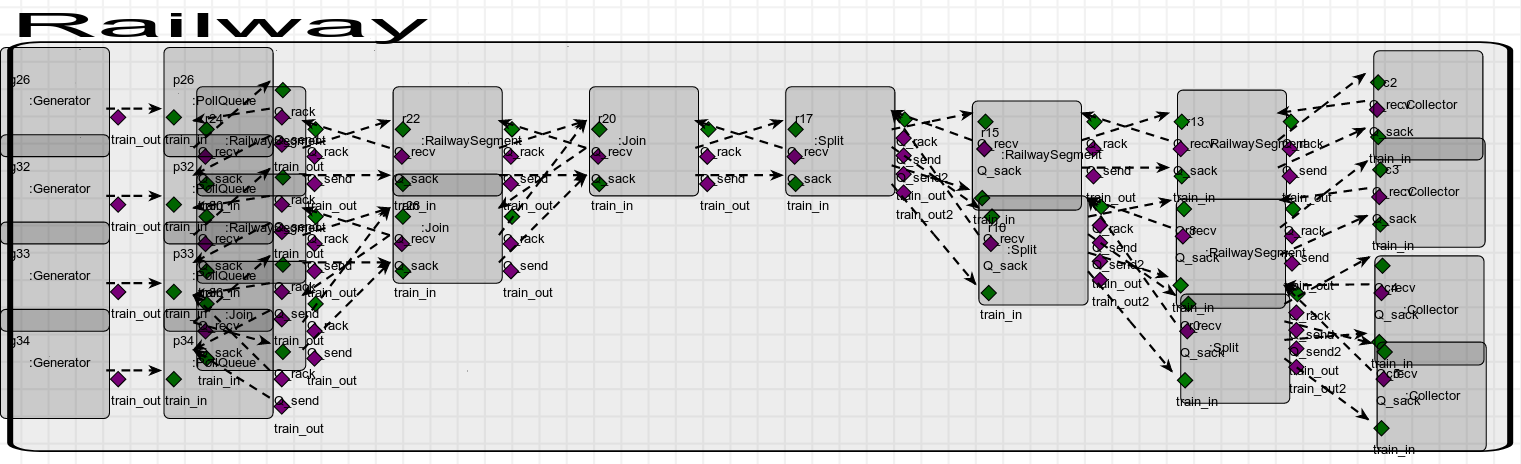
\includegraphics[width=0.8\paperwidth]{images/example_devs_devs.png}}
    \end{center}
    \caption{Intermediate coupled DEVS model}
    \label{example_devs_devs}
\end{figure}

Similarly to the safety analysis, we create an intermediate coupled DEVS model here (figure \ref{example_devs_devs}. This we can then use to simulate the whole railway system and retrieve the necessary statistics.

\begin{figure}[H]
    \begin{center}
        \makebox[\textwidth]{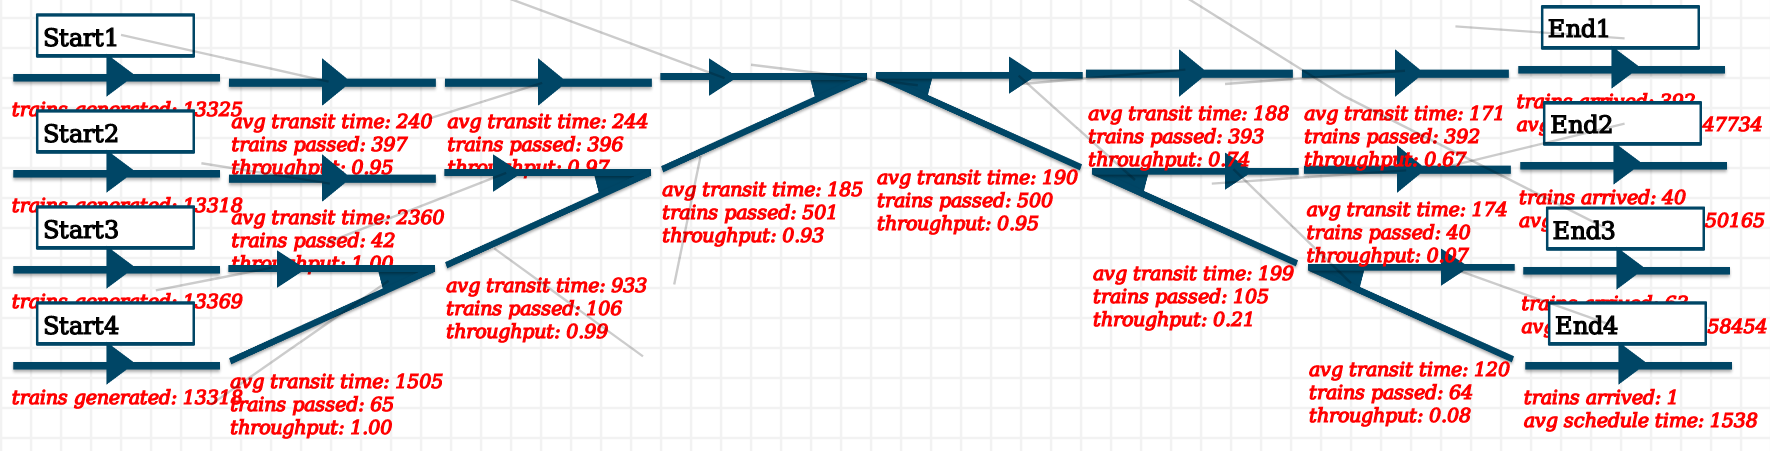
\includegraphics[width=0.8\paperwidth]{images/example_devs_results.png}}
    \end{center}
    \caption{Queueing analysis results}
    \label{example_devs_results}
\end{figure}

Looking at the results, we immediately see that the middle junction and turnout have a high throughput, meaning a lot of traffic (in fact, all traffic) goes through this point. Another shocking fact is that only one train from schedule 4 (\texttt{Start4} - \texttt{End4}) has arrived at their end station and that most of the trains that finished are from schedule 1. Furthermore, we can conclude that the tracks starting from \texttt{Start1} have a high throughput and a low transit time which is desirable. On the other hand, the tracks starting from \texttt{Start4} also have a high throughput (approx. 100\% even), but they have an extremely long transit time since the trains probably have to wait for the other ones. Judging from this, there is some kind of indirect priority system (probably due to the pseudo-randomness), i.e. trains from schedule 1 have the most priority.

\end{document}
